\documentclass[9pt]{beamer}

\usepackage[T1]{fontenc}
\usepackage{color}
\usepackage{graphicx}
\usepackage{natbib}
\usepackage{tikz}
\usepackage{xmpmulti}
\usepackage{animate}

\usetheme{Boadilla}
\usetheme{Hannover}

\usefonttheme{professionalfonts}

\title[Apsis Tools]{Automated evidence synthesis for climate change mitigation}
\subtitle{}
\author{Max Callaghan}
\institute[MCC]{
	%
\includegraphics[height=1cm,width=2cm]{/home/max/Pictures/MCC_Logo_RZ_rgb.jpg}
	
\includegraphics[height=1cm,width=2cm]{MCC_Logo_RZ_rgb.jpg} \hspace{0.5cm}
	
\includegraphics[height=1cm]{images/leeds_logo.jpg}	
	\medskip
	
	\large
	
	The Mercator Research Institute on Global Commons and Climate Change
	
	\medskip
	
	The Priestley International Centre for Climate, University of Leeds
}
\newtheorem*{remark}{}

\bibliographystyle{apalike}



%\begin{frame}{Climate change - a wicked problem}
%
%\begin{columns}
%	\begin{column}{0.5\linewidth}
%		content...
%	\end{column}
%	\begin{column}{0.5\linewidth}
%		content...
%	\end{column}
%\end{columns}
%
%\end{frame}

\begin{document}
	
\AtBeginSection[]
{
	\begin{frame}<beamer>
	\frametitle{Outline}
	\tableofcontents[currentsection]
\end{frame}
}
	
\begin{frame}
	\titlepage
\end{frame}

% Context
% IPCC
% Big literature
% Systematic review
% Automation and systematic review
% Two threads joined together
% Platform
% NETs
% Cities
% Topography
% Automation
% - Screning
% - Classification

\begin{frame}{Outline}

\tableofcontents

\end{frame}

\section{Context}

\begin{frame}{Climate change - a wicked problem}

Climate change is 

\begin{itemize}
	\item<1-> complex
	\item<2-> uncertain
	\item<3-> value laden
\end{itemize}


%
%\begin{columns}
%	\begin{column}{0.5\linewidth}
%		content...
%	\end{column}
%	\begin{column}{0.5\linewidth}
%		content...

%	\end{column}
%\end{columns}

\end{frame}

\begin{frame}{The IPCC}

\begin{columns}
	\begin{column}{1\linewidth}
		\begin{figure}
			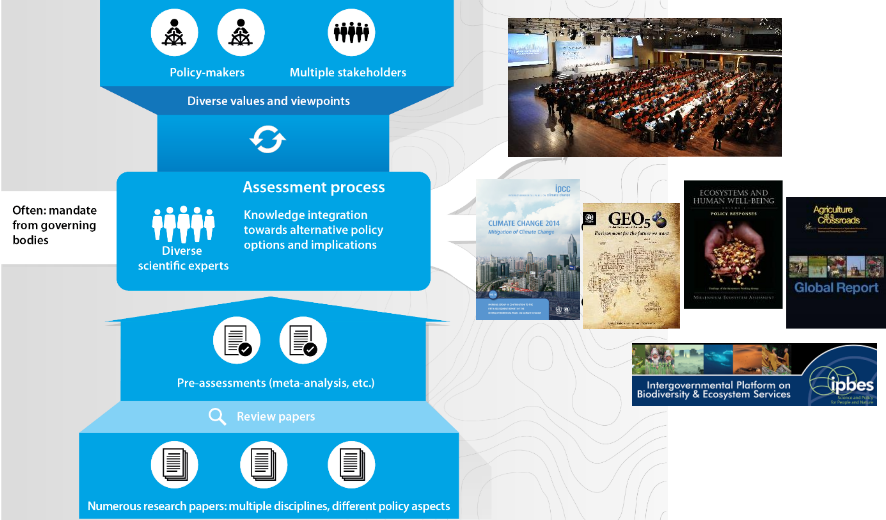
\includegraphics[width=0.9\linewidth]{images/assessments_pyramid.png}
		\end{figure}
	\end{column}
%	\begin{column}{0.5\linewidth}
%		content...
%	\end{column}
\end{columns}
\begin{itemize}
	\item 
\end{itemize}

\end{frame}

\begin{frame}{The IPCC}

\begin{figure}
	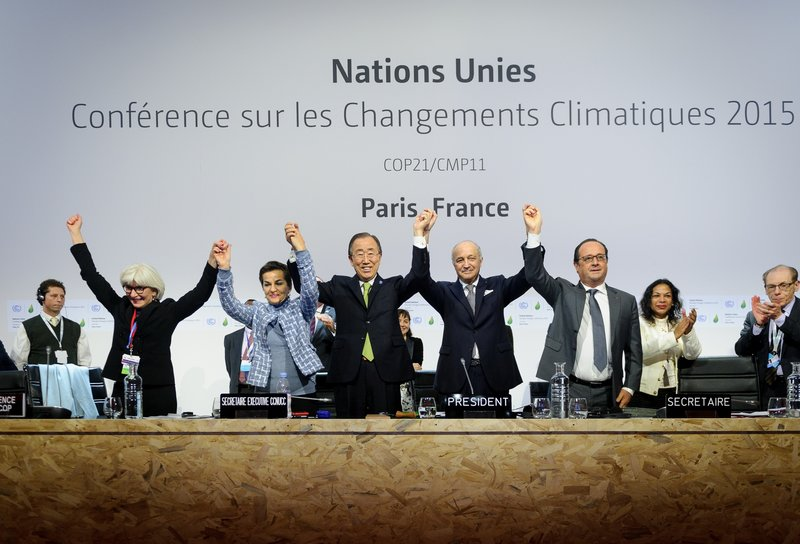
\includegraphics[width=\linewidth]{images/paris.jpg}
\end{figure}

\end{frame}

% now to the problem, as we have identified it, in our field. Though
% there are surely parallels with what is going on in your areas
\section{Problem}

\begin{frame}{Limited learning in the IPCC}

\begin{columns}
	\begin{column}{1\linewidth}
		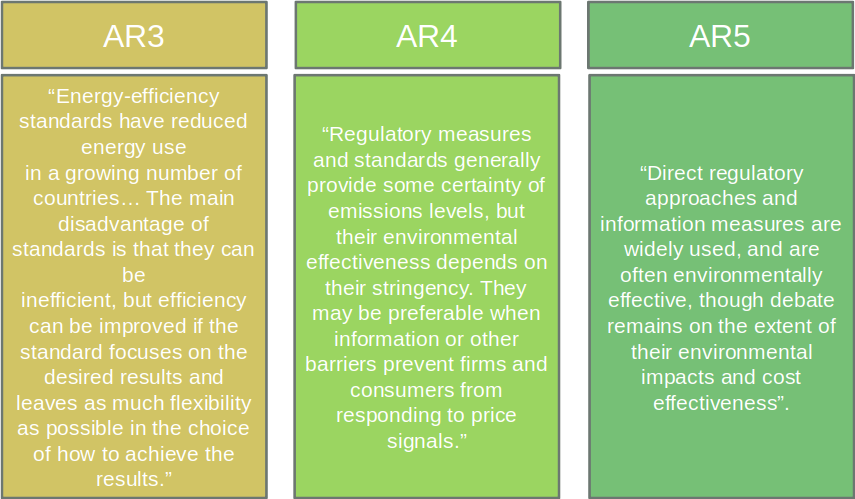
\includegraphics[width=\linewidth]{images/learning_climate.png}
	\end{column}
%	\begin{column}{0.5\linewidth}
%		content...
%	\end{column}
\end{columns}
 
\end{frame}

\begin{frame}{Big Literature}

	\begin{figure}
		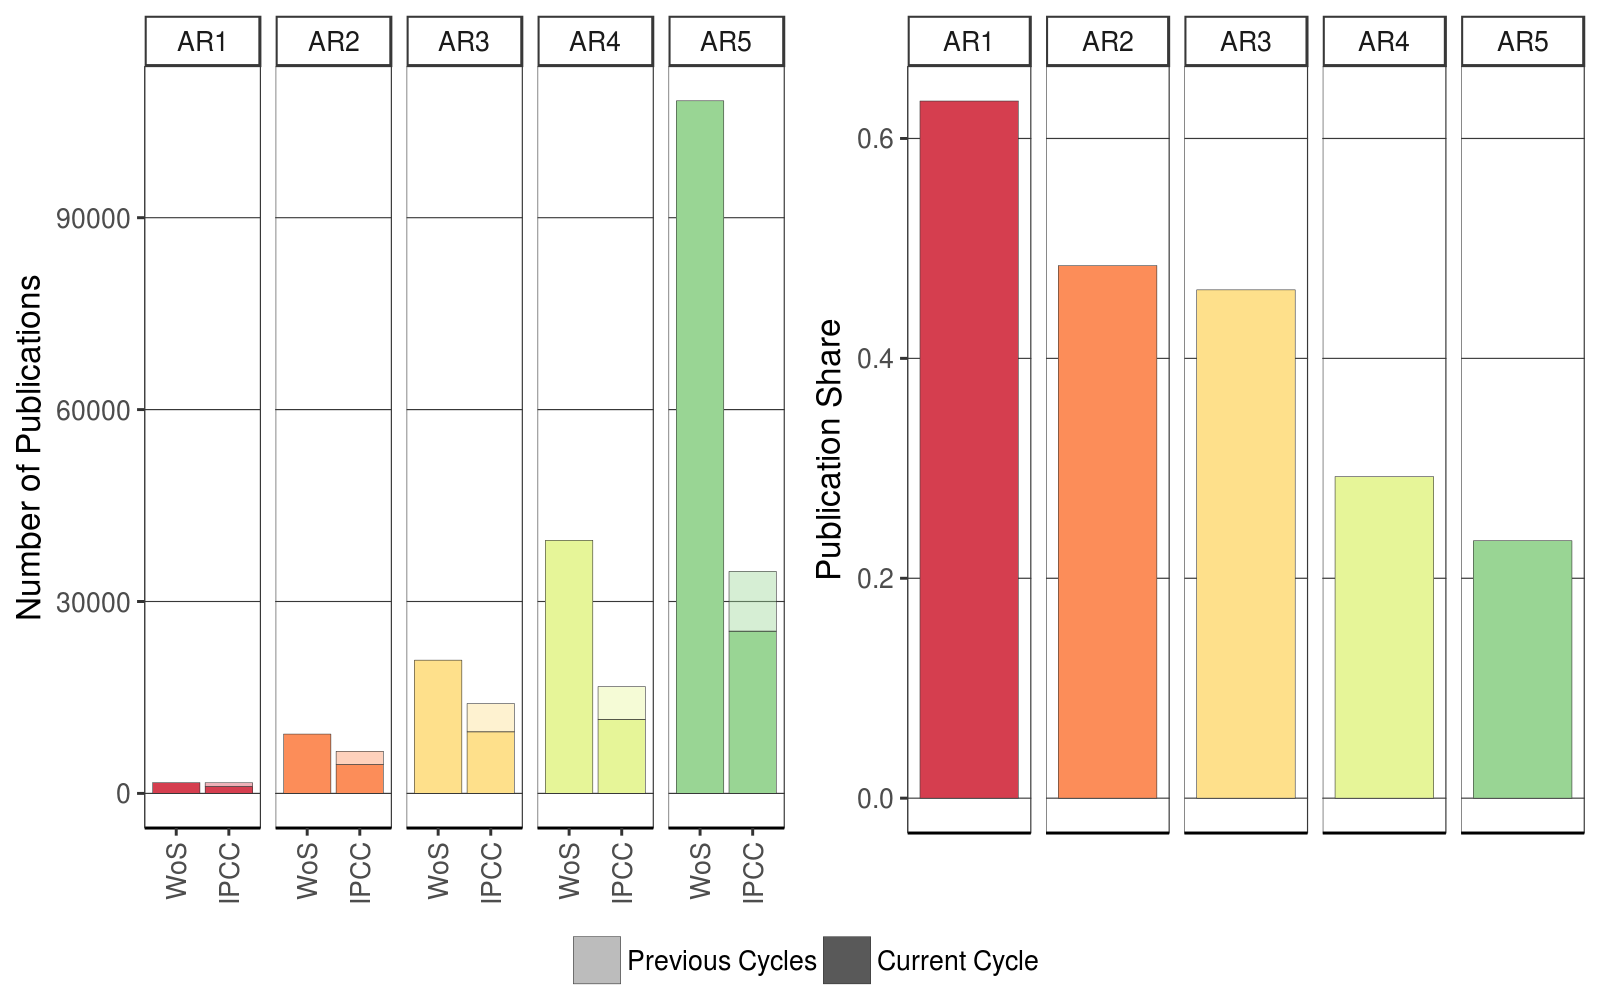
\includegraphics[width=\linewidth]{images/merged_IPCC_spectral}
		\caption{\citep{Minx2017l}}
	\end{figure}

\end{frame}

\begin{frame}{The IPCC process}

\begin{figure}
	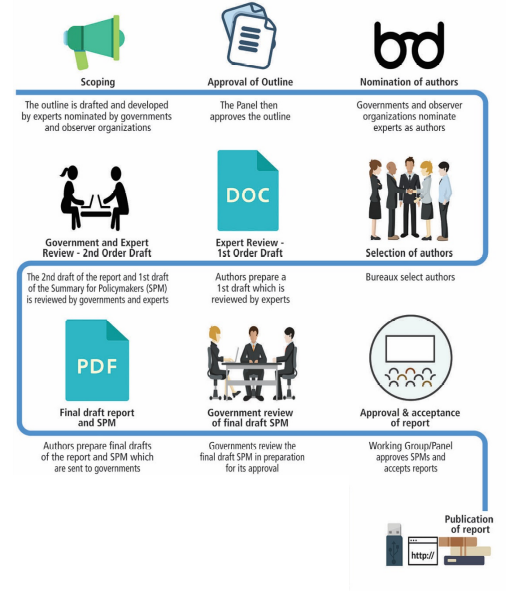
\includegraphics[width=0.6\linewidth]{images/ipcc_process.png}
\end{figure}

\end{frame}


\section{Our approach so far}

\begin{frame}{Implications}

	\begin{itemize}
		\item<1-> We need to develop ways of being more systematic in engaging with the literature
		\item<2-> We need more research on research results - What works, why and in what contexts?
		\item<3-> We need ways of engaging with more text than we can read ourselves
	\end{itemize}

\end{frame}

\begin{frame}{APSIS} % Our approach
% We started doing things, and I started building things
% photo Jan
\begin{columns}
	\begin{column}{0.6\linewidth}
		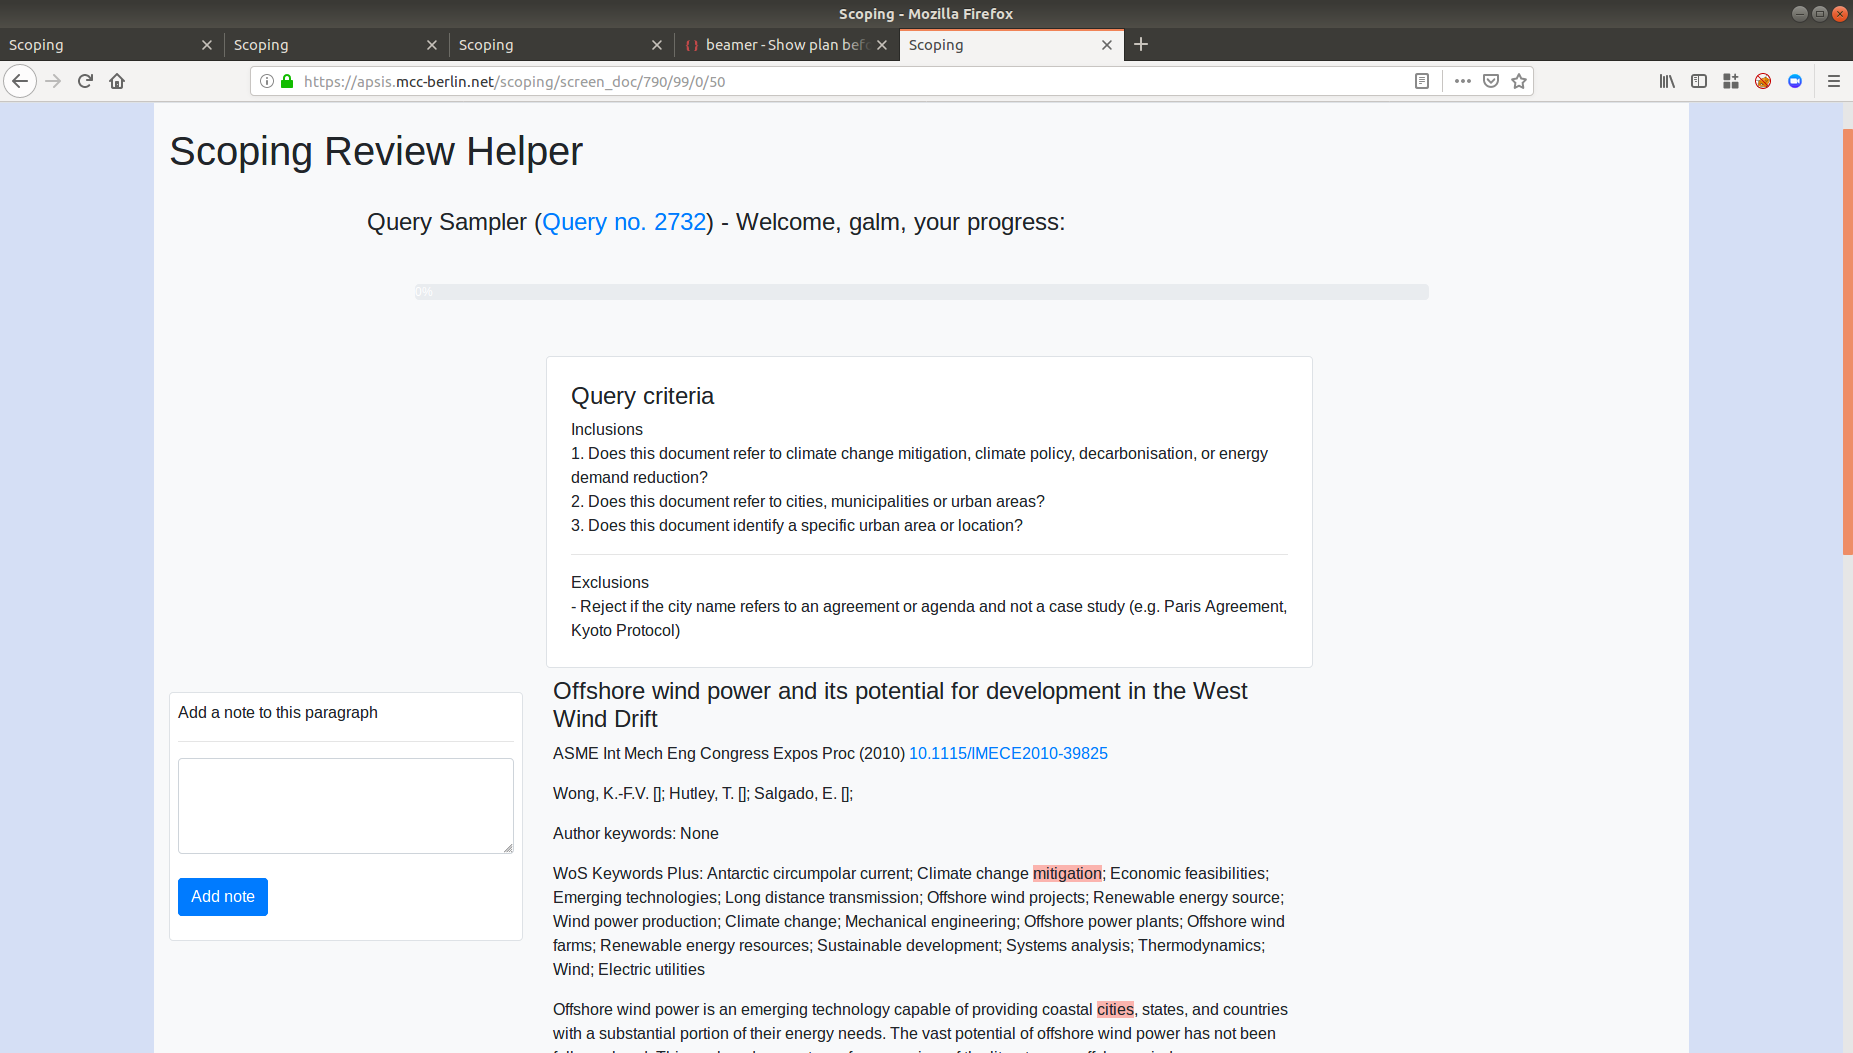
\includegraphics[width=\linewidth]{images/screenshot_apsis}
	\end{column}
	\begin{column}{0.4\linewidth}
		\textbf{Online platform}
		\begin{itemize}
			\item Django [link] web app. Extension of topic modelling visualisation app \citep{Chaney2012}
			\item Lots of data collection, analysis and exploration available through online web interface
			\item More detailed analysis made easier through structured access to data
		\end{itemize}
	\end{column}
\end{columns}

\end{frame}

\begin{frame}{Negative emissions technologies (NETs)}

\begin{columns}
	\begin{column}{0.4\linewidth}
		\begin{itemize}
			\item<1-> NETs describe technologies which remove carbon from the atmosphere and store it
			\item<2-> NETs (of one sort or another) are indispensable for reaching the 1.5 degree target
			\item<3-> We produced a quick landscape of the literature using topic modelling \citep{minx2017negative} 
		\end{itemize}
	\end{column}
	\begin{column}{0.6\linewidth}
		\begin{figure}
			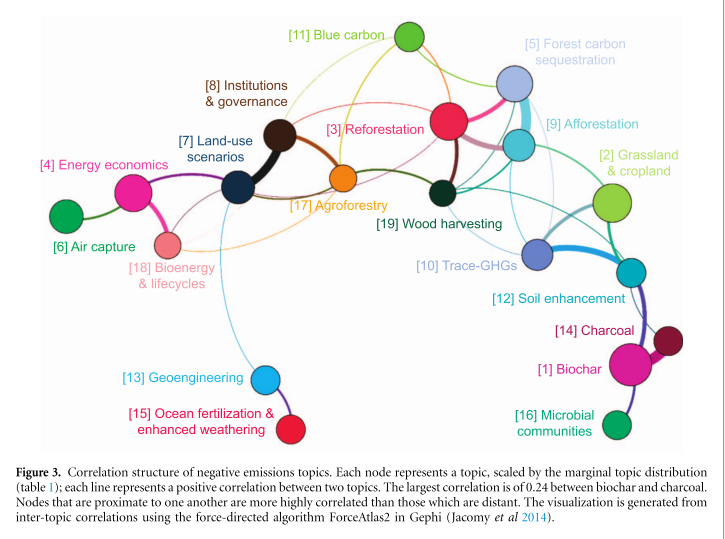
\includegraphics[width=\linewidth]{images/croissant.PNG}<3->
		\end{figure}
		
	\end{column}
\end{columns}

\end{frame}

\begin{frame}{NETs 2 - systematic review - process digitalisation}

\begin{columns}
	\begin{column}{0.5\linewidth}
		\begin{figure}
			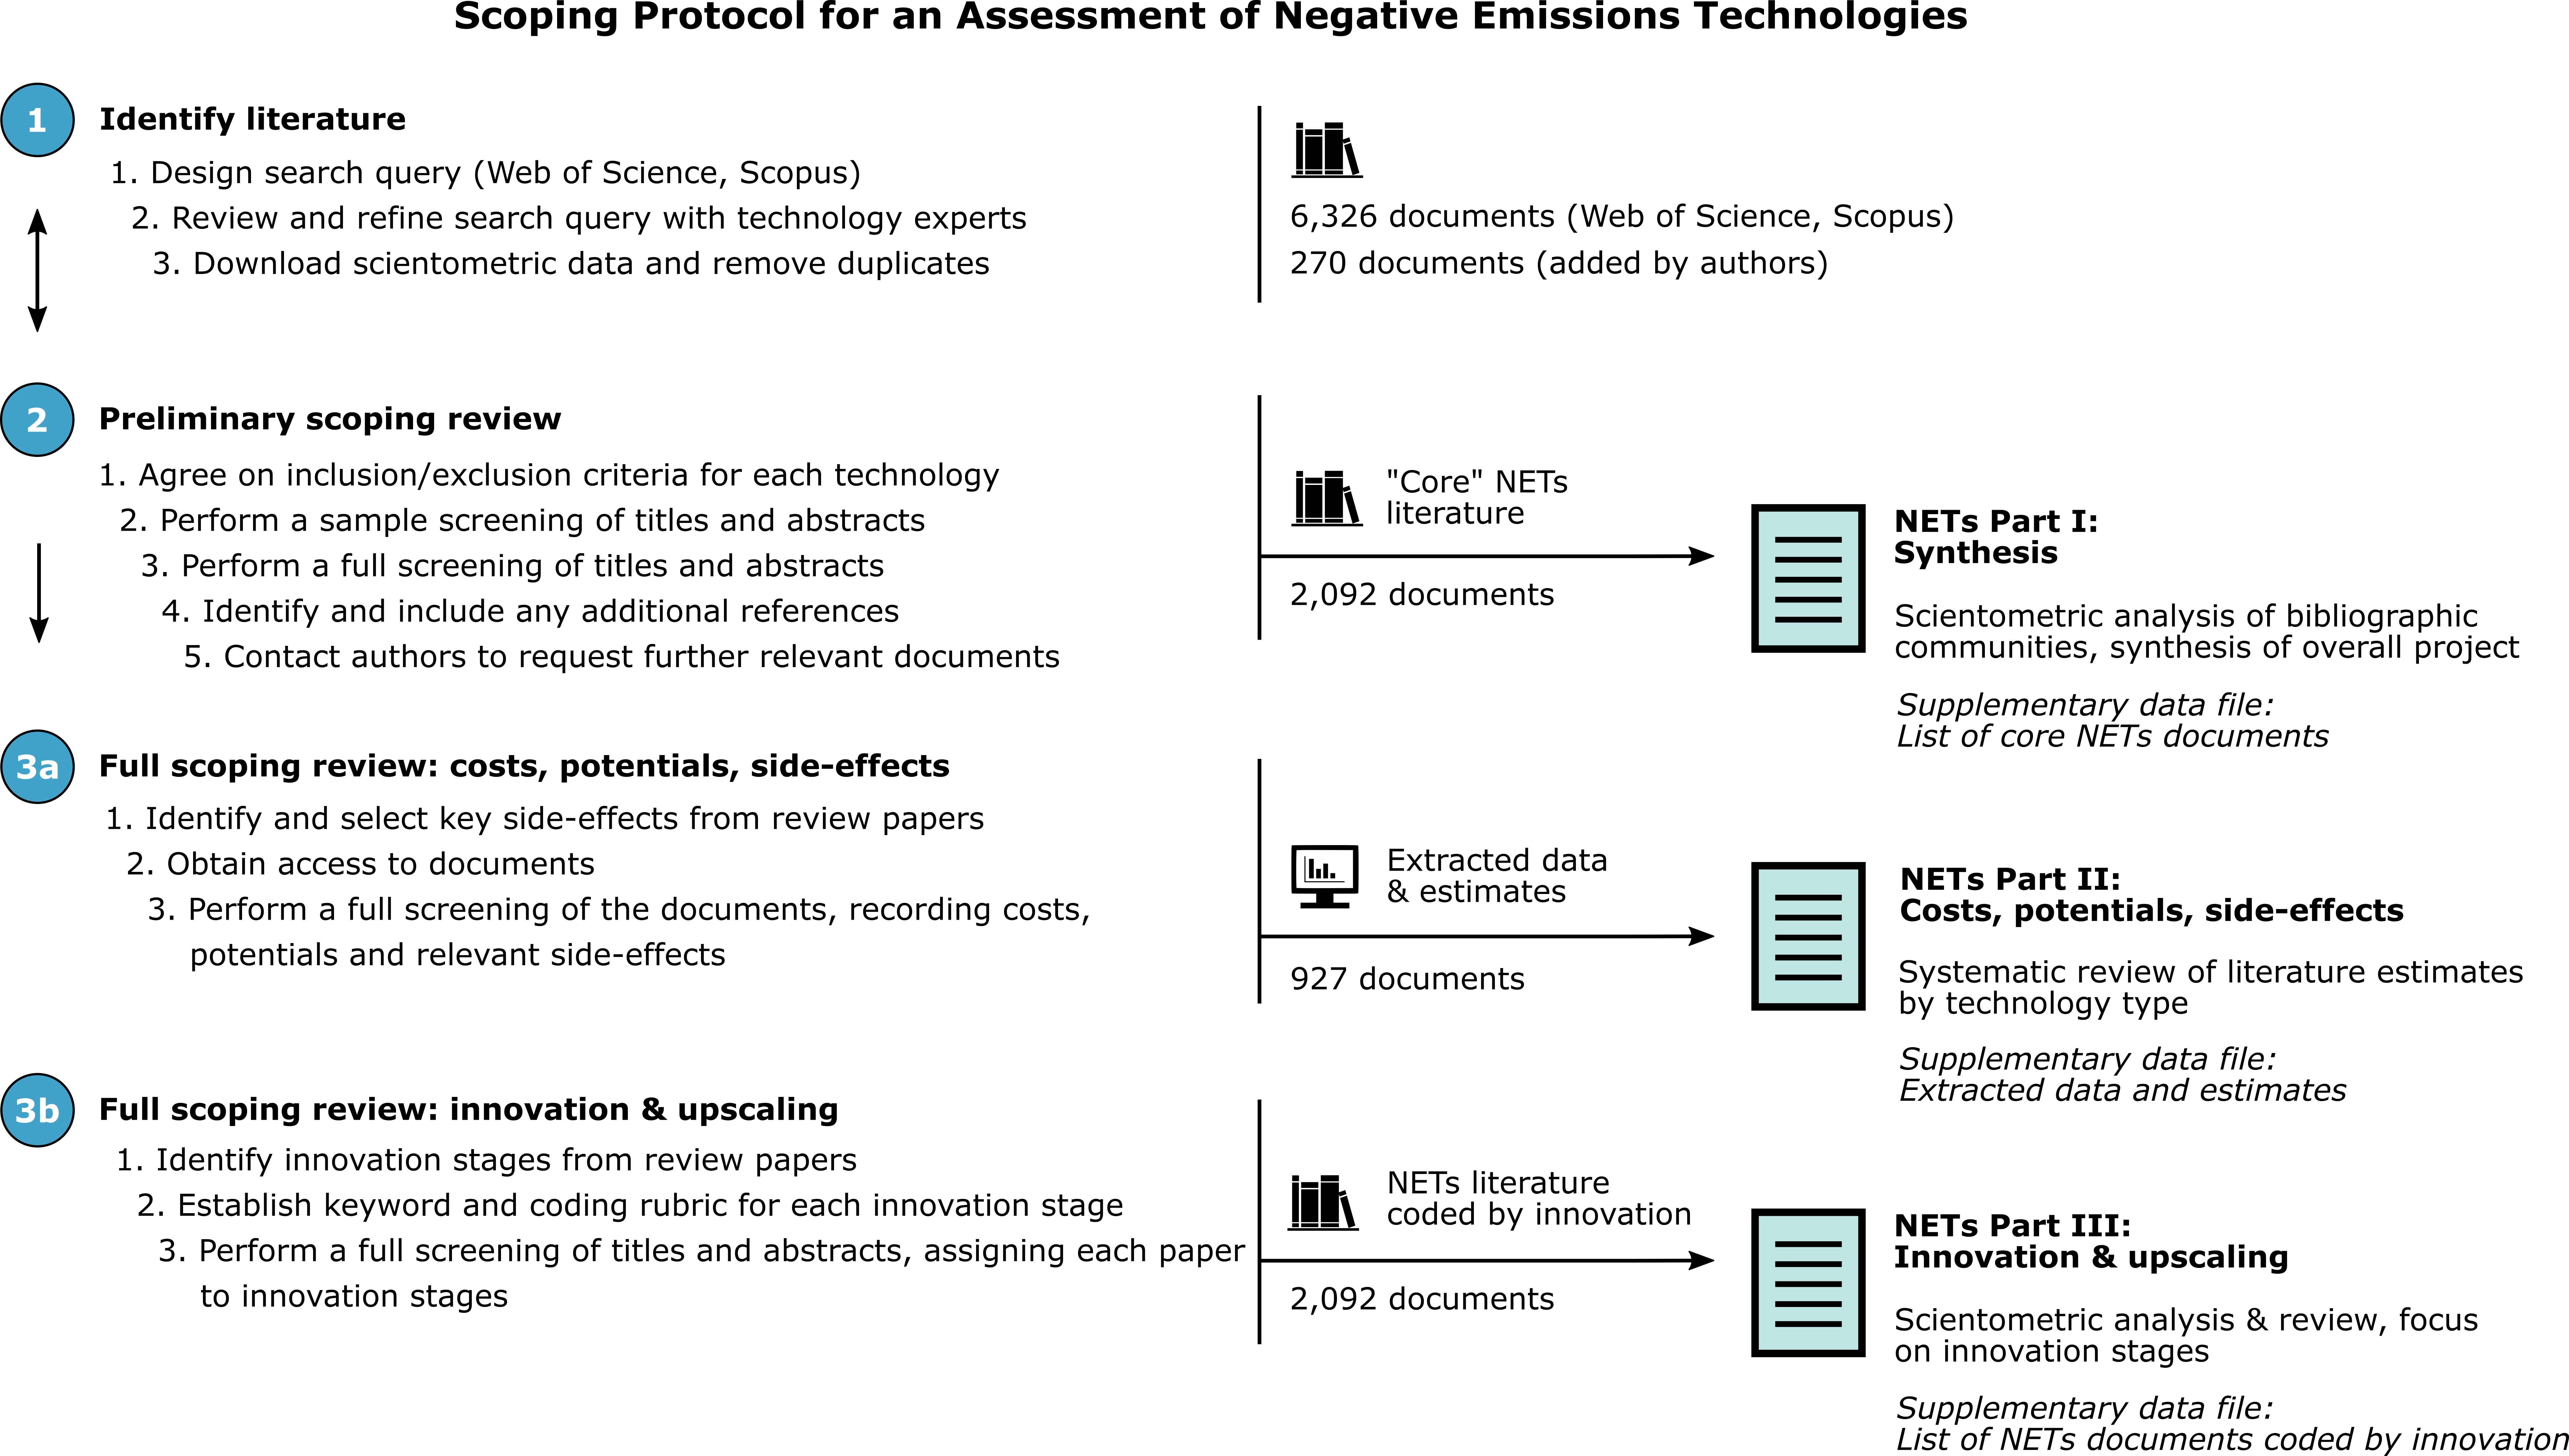
\includegraphics[width=\linewidth]{images/Fig3_scoping_protocol.png}
		\end{figure}
	\end{column}
	\begin{column}{0.5\linewidth}
		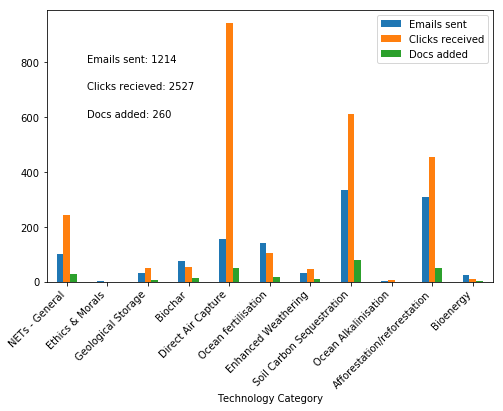
\includegraphics[width=\linewidth]{images/emails_responses.png}
	\end{column}
\end{columns}

% picture of documents at each stage
% Emails
% Map
% heatbars

\end{frame}

\begin{frame}{NETs 2 - systematic review - Results}
	\begin{columns}
		\begin{column}{0.5\linewidth}
			\begin{figure}
				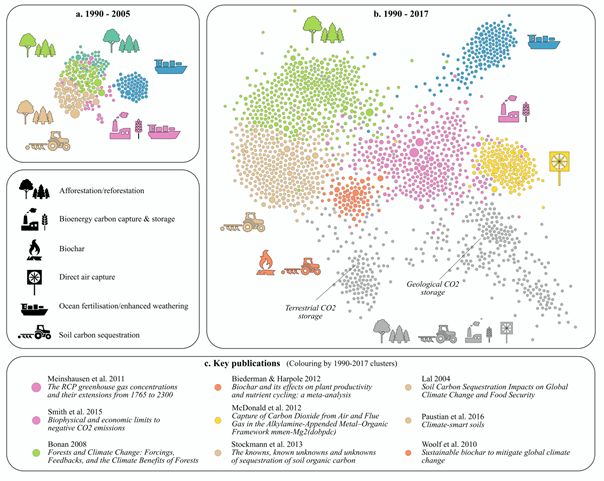
\includegraphics[width=\linewidth]{images/NETs_network.png}
			\end{figure}
		\end{column}
		\begin{column}{0.5\linewidth}
			\begin{figure}
				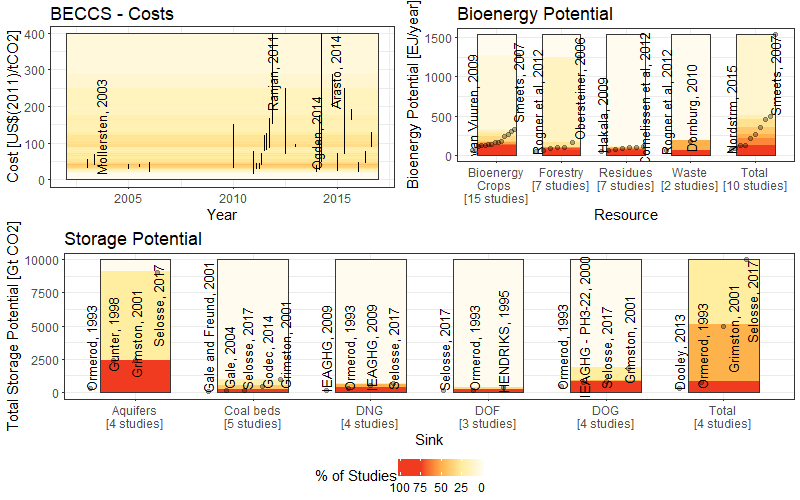
\includegraphics[width=\linewidth]{images/panel.png}
			\end{figure}
		\end{column}
	\end{columns}
\end{frame}

\begin{frame}{Urban mitigation research on cities}

\begin{figure}
	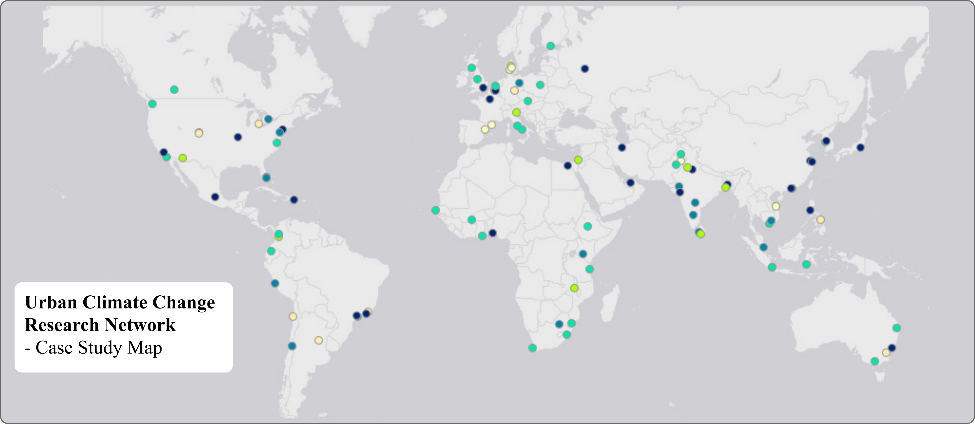
\includegraphics[width=0.8\linewidth]{images/empty_map}<1->
	
\end{figure}

\begin{figure}
	
	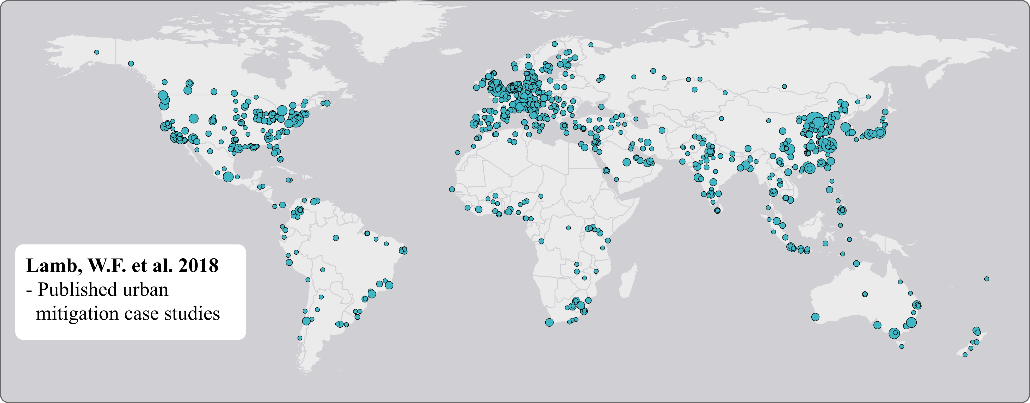
\includegraphics[width=0.8\linewidth]{images/full_map}<2->
\end{figure}

\end{frame}

\begin{frame}{Urban mitigation research on cities}

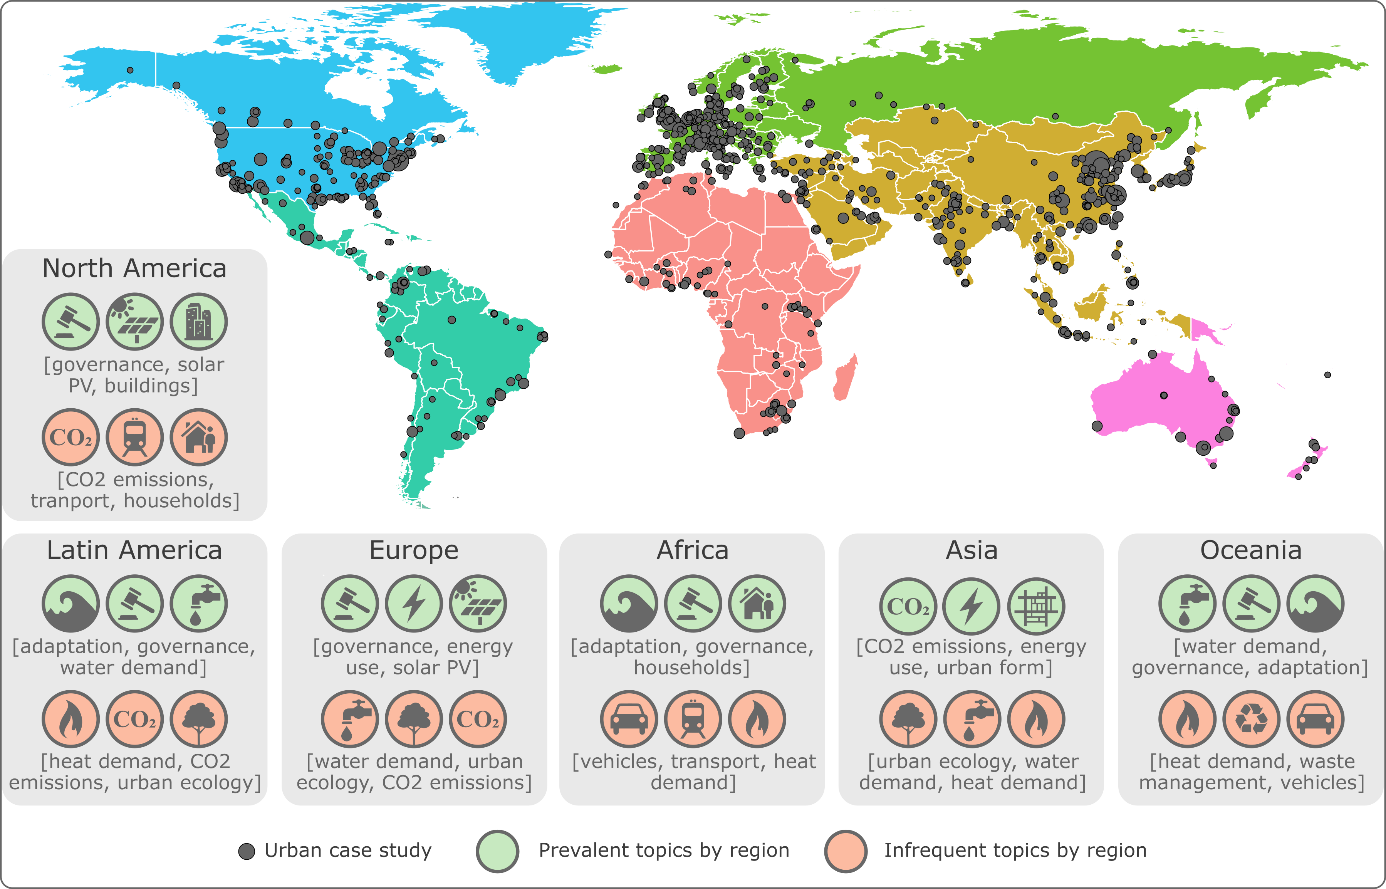
\includegraphics[width=\linewidth]{images/city_topics_map}

\citep{Lamb2018a}

\end{frame}

\section{Ongoing work}

%\begin{frame}
%	\tableofcontents
%\end{frame}

\begin{frame}{A topography of climate change literature}

\begin{columns}
	\begin{column}{0.5\linewidth}
		\begin{figure}
			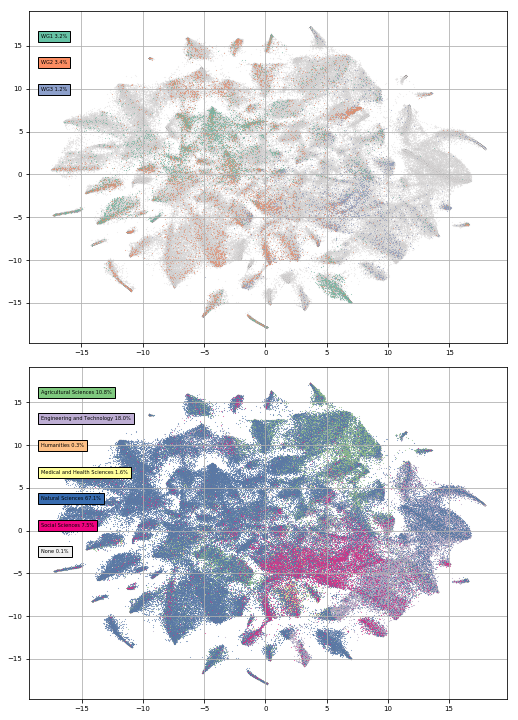
\includegraphics[width=\linewidth]{images/run_665_s_0_p200_double}
		\end{figure}
	\end{column}
	\begin{column}{0.5\linewidth}
		\begin{itemize}
			\item What's the literature on climate change \textit{about}
			\item How have topics evolved
			\item How are topics represented in IPCC reports
		\end{itemize}
	\end{column}
\end{columns}



\end{frame}

% some remarks on maps.
% A systematic map is not the same as a topography or a landscape
% but they are part of the same process and can be complementary
\begin{frame}{Machine assisted screening}

\begin{columns}
	\begin{column}{0.3\linewidth}
		\begin{itemize}
			\item<1-> For a landscape paper on ``sustainability'' we want to look at around 200,000 papers
			\item<2-> Some papers in medical/psychology/business fields use sustainable in a literal sense
			\item<3-> We have relevant/irrelevant results in our dataset, but no resources to classify them (all) by hand
		\end{itemize}
	\end{column}
	\begin{column}{0.4\linewidth}
		\begin{figure}
			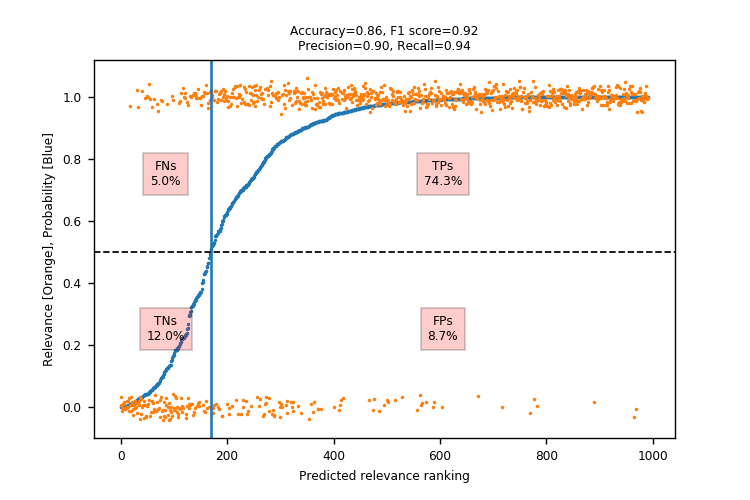
\includegraphics[width=\linewidth]{images/example.png}<4->
		\end{figure}
		\begin{itemize}
			\item<5-> We have experimented with standard text classification approaches

		\end{itemize}
	\end{column}
	\begin{column}{0.3\linewidth}
		\begin{itemize}
			\item<6-> Each use case for machine learning is specific -> recipes/frameworks for analysis and evaluation
			\item<7-> \textit{What} (not just how much) is being misclassified
		\end{itemize}
	\end{column}
\end{columns}

\end{frame}


\begin{frame}{Machine assisted classification}

Validating topic models \textit{as systematic maps} against human classification. [Unsupervised/semi-supervised]

\bigskip

Using human classifications to train a model to predict study class. [supervised]

\end{frame}


\begin{frame}{References}

callaghan@mcc-berlin.net

\medskip

%\scriptsize

Our systematic review app: \url{https://github.com/mcallaghan/tmv} 

\medskip


\medskip


%\bibliography{/home/max/ownCloud/applications/pubs/mypubs}
\bibliography{/home/max/Documents/library/library}
\end{frame}


\end{document}



\end{document}